\documentclass[aspectratio=169]{beamer}
\usetheme{metropolis}

\usepackage[utf8]{inputenc}
\usepackage[english]{babel}
\usepackage{amsmath}
\usepackage{amsfonts}
\usepackage{booktabs}
\usepackage{listings}

% Configuración para bloques de código Python
\lstset{
	language=Python,
	basicstyle=\ttfamily\footnotesize,
	keywordstyle=\color{blue},
	commentstyle=\color{green!50!black},
	stringstyle=\color{orange},
	breaklines=true,
	frame=single,
	showstringspaces=false
}

\title{Attention Mechanisms}
\subtitle{The Core of the Transformer Architecture}
\author{Juan Irving Vasquez}
\date{\today}
\institute{Instituto Politécnico Nacional (IPN)}
\titlegraphic{
\includegraphics[height=1.2cm]{ipn-cidetec.png}\hspace{0.1cm}
\includegraphics[height=1.2cm]{escudoESCOM}}

\begin{document}
	
	\maketitle
	
	% --- Diapositiva 1: Why Attention? ---
	\begin{frame}{The Motivation for Attention}
		\begin{itemize}
			\item The task
		\end{itemize}
		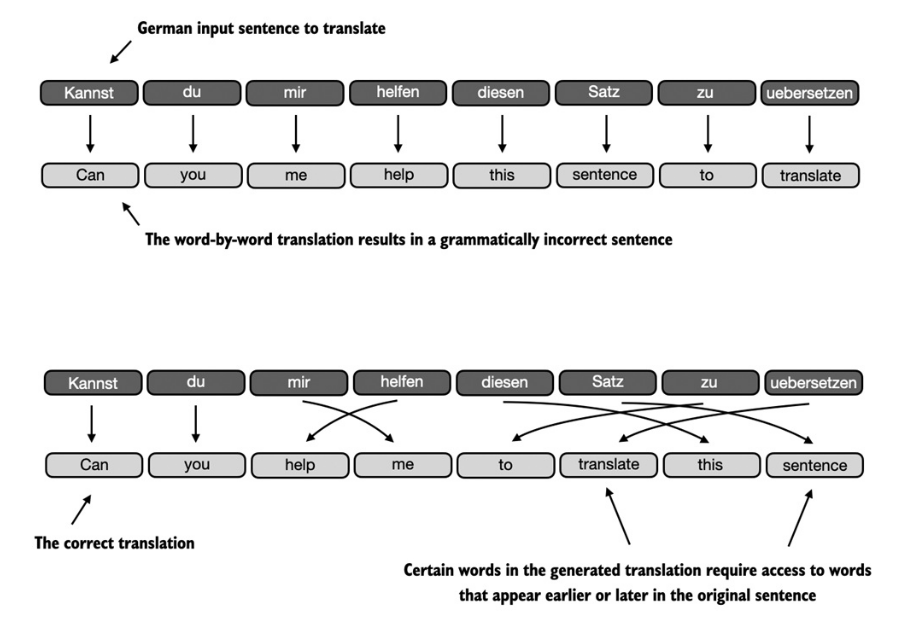
\includegraphics[height=0.8\textheight]{long_sequence}
	\end{frame}


	% --- Diapositiva 1: Why Attention? ---
	\begin{frame}{The Motivation for Attention}
		\begin{itemize}
			\item \textbf{Problem with RNNs:} Difficulty in capturing long-range 		\end{itemize}
		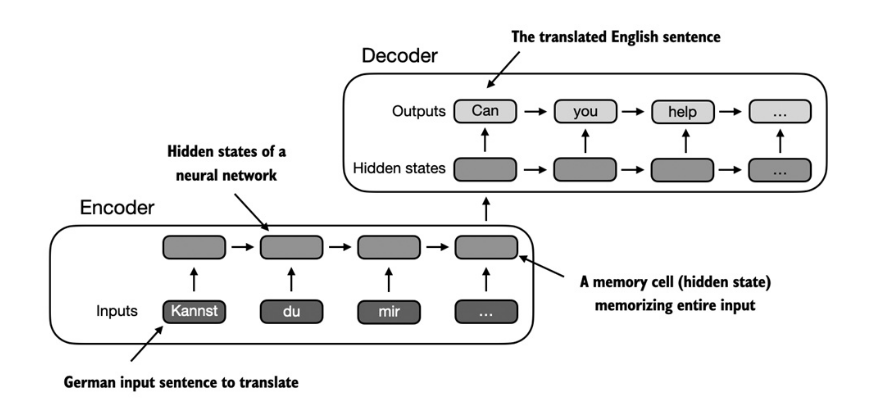
\includegraphics[height=0.8\textheight]{rnn}
	\end{frame}
	
	% --- Diapositiva 1: Why Attention? ---
	\begin{frame}{The Motivation for Attention}
		\begin{itemize}
			\item \textbf{The Attention Concept:} Allows the model to focus on different parts of the input sequence regardless of their distance.
			\item \textbf{Key Insight:} Instead of a fixed-size hidden state, we compute a weighted sum of all input tokens' representations.
		\end{itemize}
	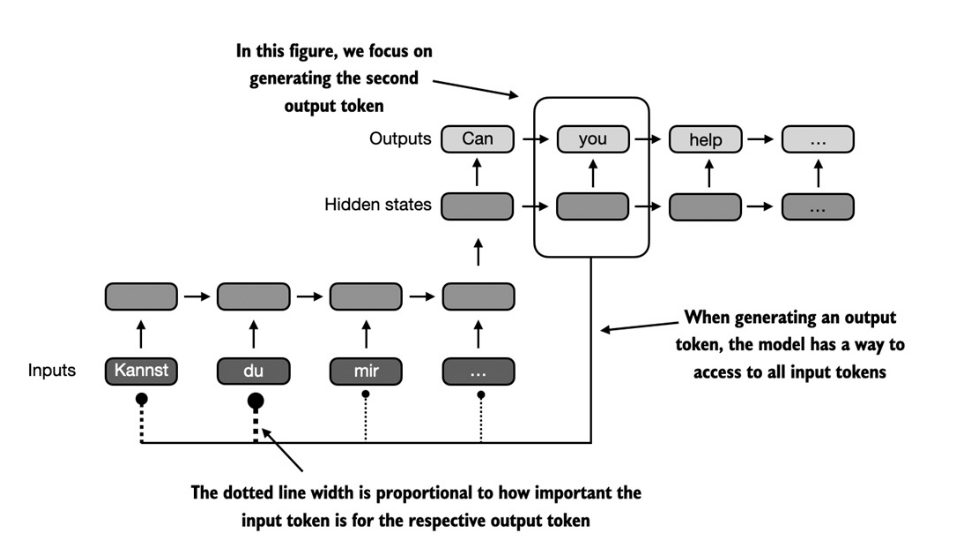
\includegraphics[height=0.6\textheight]{focusing}
	\end{frame}


	\frame{
		\frametitle{The paper that made the revolution}
		%\begin{figure}
		\centering
		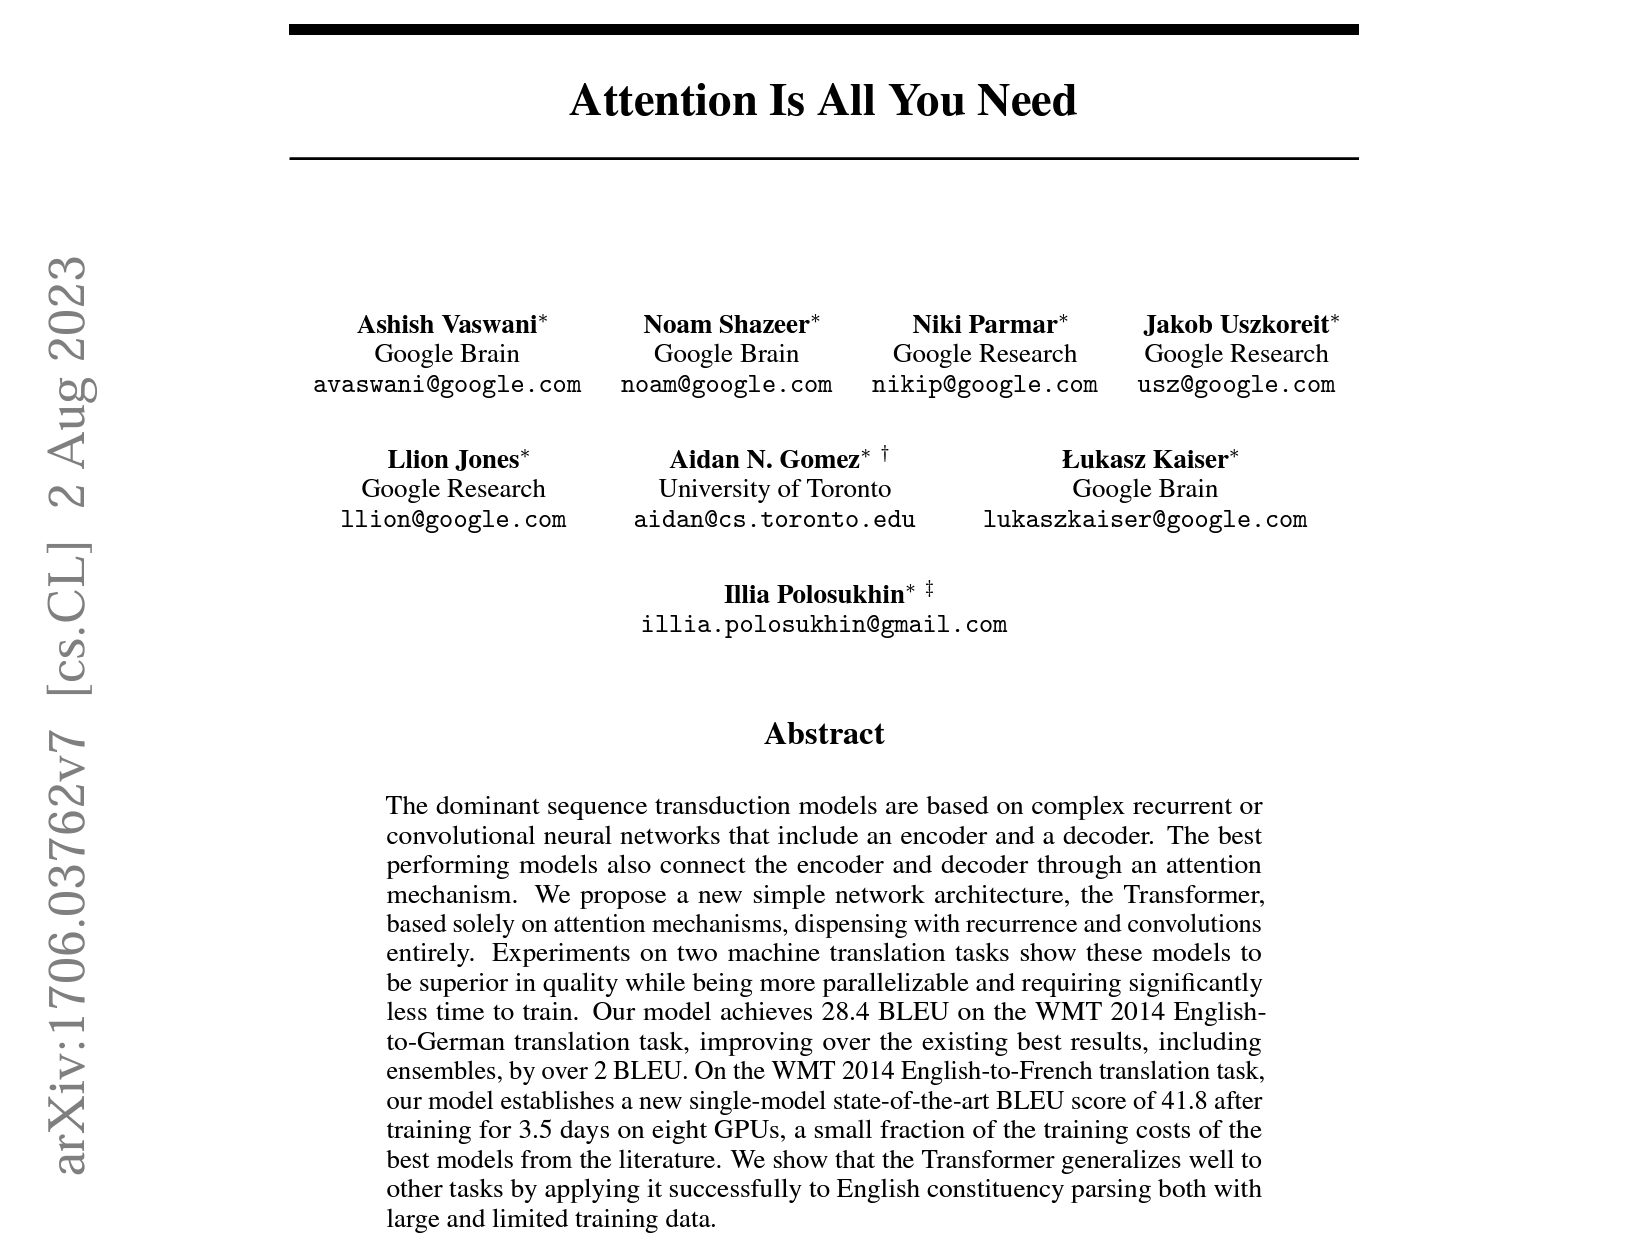
\includegraphics[width=0.6\linewidth]{aisyn}
	}


	\begin{frame}
		\frametitle{The transformer architecture}
		\begin{figure}
			\centering
			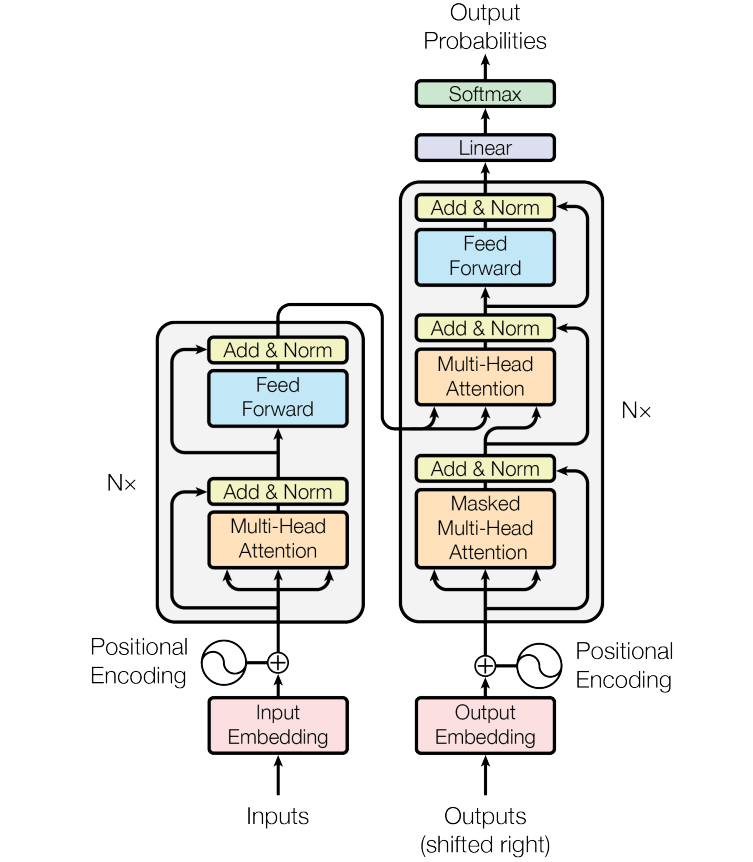
\includegraphics[height=0.8\textheight]{transformer}
			%\caption{}
			%\label{fig:transformer}
		\end{figure}
	\end{frame}


	\begin{frame}
		\frametitle{Attention mechanism (Vaswani et al. 2017)}
		\begin{figure}
			\centering
			\includegraphics[height=0.75\textheight]{"scaled dot product"}
			\caption{Scaled dot-product attention}
			\label{fig:scaled-dot-product}
		\end{figure}
	\end{frame}

	
	% --- Diapositiva 2: Scaled Dot-Product Attention ---
	\begin{frame}{Scaled Dot-Product Attention: The Math}
		The core operation involves three learnable matrices: \textbf{Query (Q)}, \textbf{Key (K)}, and \textbf{Value (V)}.
		
		\begin{equation}
			\text{Attention}(Q, K, V) = \text{softmax}\left( \frac{QK^T}{\sqrt{d_k}} \right)V
		\end{equation}
		
		\begin{itemize}
			\item \textbf{Dot-Product ($QK^T$):} Measures similarity between queries and keys.
			\item \textbf{Scaling ($1/\sqrt{d_k}$):} Prevents the softmax from entering regions with extremely small gradients when $d_k$ is large.
			\item \textbf{Softmax:} Normalizes scores into probabilities (weights summing to 1).
		\end{itemize}
	\end{frame}
	
	% --- Diapositiva 3: Self-Attention vs. Cross-Attention ---
	\begin{frame}{Self-Attention vs. Cross-Attention}
		\begin{columns}
			\column{0.5\textwidth}
			\textbf{Self-Attention:}
			\begin{itemize}
				\item $Q, K, V$ all originate from the same input sequence.
				\item Used in Encoders and Decoders to relate different positions of the same sequence.
			\end{itemize}
			
			\column{0.5\textwidth}
			\textbf{Cross-Attention:}
			\begin{itemize}
				\item $Q$ comes from one sequence (e.g., decoder), while $K$ and $V$ come from another (e.g., encoder output).
				\item Essential for tasks like Machine Translation.
			\end{itemize}
		\end{columns}
	\end{frame}
	
	
	% --- Diapositiva 4: Causal Attention (Masking) ---
	\begin{frame}[fragile]{Causal Attention: Masking the Future}
		In GPT-like models (Decoder-only), a token should only attend to previous tokens.
		\begin{itemize}
			\item \textbf{Implementation:} Apply a triangular mask (lower triangular matrix) to the scores before the softmax.
			\item \textbf{Value:} Future positions are set to $-\infty$, resulting in 0 probability after softmax.
		\end{itemize}
	\end{frame}

	
	% --- Diapositiva 5: Multi-Head Attention (MHA) ---
	\begin{frame}{Multi-Head Attention (MHA)}
		Why use multiple heads?
		\begin{itemize}
			\item Allows the model to jointly attend to information from different representation subspaces at different positions.
			\item \textbf{Process:} 
			\begin{enumerate}
				\item Split $Q, K, V$ into $h$ heads.
				\item Perform attention in parallel.
				\item Concatenate the results and apply a linear projection.
			\end{enumerate}
		\end{itemize}
		[Image of multi-head attention architecture]
	\end{frame}
	
	% --- Diapositiva 6: Computational Complexity ---
	\begin{frame}{Computational Efficiency and Complexity}
		\begin{itemize}
			\item \textbf{Self-Attention Complexity:} $O(L^2 \cdot d)$, where $L$ is sequence length and $d$ is embedding dimension.
			\item \textbf{Comparison:} 
			\begin{itemize}
				\item RNNs are $O(L \cdot d^2)$ but sequential.
				\item Transformers are parallelizable but quadratic with respect to length.
			\end{itemize}
			\item This quadratic growth is why extending the \textbf{Context Window} is a major research challenge in LLMs.
		\end{itemize}
	\end{frame}
	
	% --- Diapositiva 7: Implementation Overview ---
	\begin{frame}[fragile]{From Math to Code: PyTorch Structure}
		\begin{lstlisting}
			class MultiHeadAttention(nn.Module):
			def __init__(self, d_in, d_out, context_len, dropout, num_heads):
			super().__init__()
			self.W_query = nn.Linear(d_in, d_out, bias=False)
			self.W_key = nn.Linear(d_in, d_out, bias=False)
			self.W_value = nn.Linear(d_in, d_out, bias=False)
			# ... rest of the logic
		\end{lstlisting}
		\textbf{Crucial:} Biases are often omitted in $Q, K, V$ linear layers in modern implementations to simplify the geometry of the projection.
	\end{frame}
	
	\begin{frame}[standout]
		Next Chapter: Implementing a GPT Model from Scratch
	\end{frame}
	
\end{document}